\section{Materiais e Métodos}
\label{sec:metodologia}

O desenvolvimento compreendeu a caracterização independente dos sensores,
a integração de duas unidades embarcadas e a avaliação de uma regra de
alerta com dados rotulados. O objetivo operacional foi detectar desvios
posturais sustentados e fornecer retorno por vibração. A identificação do
tipo de postura auxilia a interpretação da decisão, sem constituir uma
exigência de classificação exaustiva. Os procedimentos foram descritivos:
as campanhas de bancada, as capturas integradas, a validação com atuador
e a demonstração pública tiveram condições e finalidades distintas.

\subsection{Visão geral e arquitetura do sistema}
\label{sec:met-arquitetura}

O protótipo reuniu uma unidade vestível, posicionada na parte superior das
costas, e uma cadeira instrumentada. Ambas empregaram placas Seeed Studio
XIAO nRF52840 Sense. A unidade corporal adquiriu a orientação pelo
acelerômetro da IMU embarcada e comandou um motor vibratório. A cadeira
leu oito sensores resistivos de força FSR402, recebeu os ângulos do corpo,
armazenou a referência de calibração em memória de execução e calculou o
alerta. A Figura~\ref{fig:met-arquitetura} apresenta os caminhos de
sensoriamento, decisão, atuação e visualização.

\begin{figure}[H]
  \centering
  \caption{Arquitetura do sistema e interfaces de comunicação.}
  \label{fig:met-arquitetura}
  \begin{tikzpicture}[
    box/.style={draw,rounded corners,align=center,text width=3.25cm,
                minimum height=1.05cm,font=\small},
    arr/.style={-{Latex[length=2mm]},thick},
    note/.style={font=\footnotesize,align=center,fill=white,inner sep=2pt}]
    \node[box] (body) at (0,0) {XIAO do corpo\\aquisição da IMU e atuação};
    \node[box] (chair) at (8,0) {XIAO da cadeira\\calibração e regra de fusão};
    \node[box] (imu) at (0,2.7) {LSM6DS3TR-C\\acelerômetro};
    \node[box] (fsr) at (8,2.7) {8 FSR402 + CD74HC4067\\4 assento + 4 encosto};
    \node[box] (motor) at (0,-2.8) {Driver BC337\\motor vibratório};
    \node[box] (pc) at (8,-3.3) {Notebook\\captura e dashboard};
    \draw[arr] (imu) -- node[note,right] {I\textsuperscript{2}C} (body);
    \draw[arr] (fsr) -- node[note,right] {ADC} (chair);
    \draw[arr] (body.north east) -- node[note,above] {ESB: ângulos e estado\\20\,Hz} (chair.north west);
    \draw[arr] (chair.south west) -- node[note,below] {ACK payload: alerta,\\referência e comandos} (body.south east);
    \draw[arr] (body) -- node[note,right] {D10 / PWM} (motor);
    \draw[arr] (chair.south) -- node[note,right] {USB: CSV} (pc.north);
    \draw[arr,dashed] (chair.east) -- ++(0.8,0) |- node[note,pos=0.75,right] {beacon BLE} (pc.east);
  \end{tikzpicture}
  \fonte{Elaborado pelo autor (2026)}
\end{figure}

A cadeira foi adotada como unidade central de decisão porque concentra os
oito canais de contato e pode associá-los a cada amostra recebida do
corpo. Essa organização evita transmitir todos os FSRs para a unidade
vestível e permite registrar, por uma única conexão USB, a decisão e os
dados que a fundamentaram. O notebook atua como observador e ferramenta
de captura; o processamento do alerta e o acionamento do motor permanecem
autônomos. Na ausência do enlace, o corpo conserva a última referência
recebida e utiliza uma regra local baseada somente na IMU.

Os programas embarcados encontram-se em \texttt{firmware/body} e
\texttt{firmware/chair}. O protocolo e as regras compartilhadas estão em
\texttt{firmware/libraries/PostureLink}. A descrição a seguir corresponde
à implementação final consultada, enquanto as versões usadas nos
experimentos são identificadas na Seção~\ref{sec:met-experimentos}.
Essa distinção é necessária porque o controle do motor e a interface BLE
foram aperfeiçoados após as primeiras capturas integradas.

\subsection{Unidade vestível: aquisição inercial e atuação}
\label{sec:met-corpo}

\subsubsection{Montagem e estimativa de inclinação}

A placa XIAO nRF52840 Sense contém a IMU de seis eixos LSM6DS3TR-C. Na
montagem integrada, o conjunto foi acondicionado em um colar/invólucro,
com o sensor nas costas, logo abaixo do pescoço. Mede-se a orientação
local dessa região; não se obtém diretamente a curvatura de toda a coluna
nem um ângulo anatômico entre vértebras. A posição e a acomodação do
colar participam da medida e motivam a calibração a cada usuário e
recolocação.

Utilizou-se apenas o acelerômetro para estimar a inclinação estática.
Sejam $a_x$, $a_y$ e $a_z$ as componentes de aceleração nos eixos da placa.
Os ângulos, em graus, são calculados por
\begin{align}
 p &= \frac{180}{\pi}\operatorname{atan2}
       \left(-a_x,\sqrt{a_y^2+a_z^2}\right),
       \label{eq:met-pitch}\\
 r &= \frac{180}{\pi}\operatorname{atan2}(a_y,a_z).
       \label{eq:met-roll}
\end{align}
Os símbolos $p$ e $r$ correspondem aos campos \texttt{pitch} e
\texttt{roll}. Essas expressões usam a direção da gravidade em condições
aproximadamente estáticas e dispensam integração da velocidade angular.
Não eliminam erros por aceleração durante movimentos, deslocamento do
colar ou vibração do atuador. O giroscópio permanece desligado no
firmware final.

Na orientação física do colar utilizado, o desvio de \texttt{roll}
representa o plano sagital: negativo para a frente e positivo para trás.
O desvio de \texttt{pitch} representa a inclinação lateral: negativo para
a esquerda e positivo para a direita de quem está sentado. Essa
convenção de montagem, adotada em \texttt{Fusion.h} e nas ferramentas de
análise, prevalece sobre a interpretação genérica dos nomes dos ângulos
nos protocolos antigos de bancada.

O leitor \texttt{Lsm6Accel.h} acessa o sensor por \texttt{Wire1}, verifica
sua identificação e confere os registradores após a configuração. O
acelerômetro opera internamente a 416\,Hz, com escala de
$\pm16$\,g; a aplicação lê e transmite uma amostra a cada 50\,ms
(20\,Hz). Portanto, a taxa interna do sensor não deve ser confundida
com a taxa de registro do sistema. A leitura consulta a indicação de
dado novo e transfere os seis bytes dos três eixos em bloco, com
proteção contra atualização parcial dos registradores.

Verificam-se o retorno das transações I\textsuperscript{2}C, o número de
bytes e a plausibilidade do vetor. Um eixo saturado ou módulo inferior
a 0{,}25\,g invalida a orientação. O campo \texttt{imu} distingue
amostra válida, inicialização, erro de barramento/leitura incompleta,
ausência de dado novo e vetor inválido. Uma amostra inválida leva ângulos
\texttt{nan}, interrompe o alerta postural e aborta uma calibração em
curso, preservando uma referência anteriormente válida. Após 20 falhas
consecutivas, o corpo tenta reconfigurar o sensor, no máximo uma vez por
segundo. Esses mecanismos verificam a aquisição, sem assegurar que todo
vetor numericamente plausível represente uma postura correta.

\subsubsection{Acionamento do motor e interferência mecânica}

O motor de vibração tipo moeda, especificado no projeto para
$2{,}5$--4\,V e corrente de até 90\,mA, é alimentado pela saída
de 3{,}3\,V. Como sua corrente excede a de uma saída lógica, o pino
D10 comanda a base de um transistor NPN BC337 através de
1\,k\ohm. O emissor liga-se ao GND e o coletor ao terminal negativo
do motor. Um diodo em paralelo, com cátodo no positivo, oferece caminho
para a corrente indutiva no desligamento; um capacitor cerâmico de
33\,nF, identificado pela marcação ``333'', está associado à supressão
de ruído. O circuito é representado na Figura~\ref{fig:met-circuitos}.
\pendente{Confirmar a identificação do diodo flyback instalado; o registro
de montagem sugere 1N4148, mas sua marcação não foi confirmada.}

\begin{figure}[H]
  \centering
  \caption{Circuitos simplificados de leitura de um FSR selecionado e de acionamento do motor.}
  \label{fig:met-circuitos}
  \begin{tikzpicture}[font=\footnotesize,line width=0.6pt]
    \node[font=\small\bfseries] at (2,5.9) {(a) Canal da cadeira};
    \draw (1.2,5.1) node[above] {3{,}3\,V} -- (1.2,4.7);
    \draw (0.8,3.9) rectangle (1.6,4.7);
    \node[right] at (1.7,4.3) {FSR402};
    \draw (1.2,3.9) -- (1.2,3.5);
    \draw (0.65,2.7) rectangle (1.75,3.5);
    \node at (1.2,3.1) {mux};
    \node[right,align=left] at (1.85,3.1) {$C_n$ selecionado\\$R_{\mathrm{on}}\approx100$\,\ohm};
    \draw (1.2,2.7) -- (1.2,2.2) -- (3.4,2.2) node[right] {SIG / A0};
    \fill (1.2,2.2) circle (1.3pt);
    \draw (1.2,2.2) -- (1.2,1.8);
    \draw (0.8,1) rectangle (1.6,1.8);
    \node[right,align=left] at (1.7,1.4) {$R_{\mathrm{fixo}}$\\3{,}3\,k\ohm};
    \draw (1.2,1) -- (1.2,0.5);
    \draw (0.8,0.5) -- (1.6,0.5);
    \node[below] at (1.2,0.5) {GND};
    \begin{scope}[xshift=6.8cm]
      \node[font=\small\bfseries] at (2.4,5.9) {(b) Unidade corporal};
      \draw (2.5,5.1) node[above] {3{,}3\,V} -- (2.5,4.5);
      \draw (2.5,4) circle (0.5);
      \node at (2.5,4) {M};
      \draw (2.5,3.5) -- (2.5,2.3);
      \draw (2.1,1.7) circle (0.72);
      \draw (1.8,1.25) -- (1.8,2.15);
      \draw (1.8,1.95) -- (2.5,2.3);
      \draw[-{Latex[length=1.5mm]}] (1.8,1.5) -- (2.5,1.05);
      \draw (2.5,1.05) -- (2.5,0.5);
      \draw (2.1,0.5) -- (2.9,0.5);
      \node[below] at (2.5,0.5) {GND};
      \node[right] at (2.9,1.7) {BC337};
      \draw (-0.4,1.7) node[left,align=right] {D10\\PWM} -- (0.1,1.7);
      \draw (0.1,1.5) rectangle (1,1.9);
      \node[above] at (0.55,1.9) {1\,k\ohm};
      \draw (1,1.7) -- (1.8,1.7);
      % Diodo: anodo no coletor e catodo no positivo.
      \draw (2.5,4.9) -- (4,4.9) -- (4,4.2);
      \draw (3.75,4.2) -- (4.25,4.2);
      \draw (3.75,3.7) -- (4.25,3.7) -- (4,4.2) -- cycle;
      \draw (4,3.7) -- (4,3.1) -- (2.5,3.1);
      \node[above] at (4,4.9) {diodo};
      \draw (4,4.9) -- (5.2,4.9) -- (5.2,4.1);
      \draw (4.95,4.1) -- (5.45,4.1);
      \draw (4.95,3.9) -- (5.45,3.9);
      \draw (5.2,3.9) -- (5.2,3.1) -- (4,3.1);
      \node[above] at (5.2,4.9) {33\,nF};
      \fill (2.5,4.9) circle (1.3pt);
      \fill (2.5,3.1) circle (1.3pt);
    \end{scope}
  \end{tikzpicture}
  \fonte{Elaborado pelo autor (2026)}
\end{figure}

O comando usa PWM de oito bits. Na configuração final, a amplitude
adotada é 255 em uma escala de 0 a 255, com pulsos de 700\,ms ligados
e 300\,ms desligados durante o alerta. O teste manual dura
500\,ms e é registrado separadamente da decisão postural. O programa
só reconfigura a saída quando necessário, evitando reiniciar
continuamente a sequência PWM.

A vibração transmite-se ao acelerômetro e pode produzir excursões da
ordem de $\pm10\degree{}$, descritas no histórico da correção do motor.
Para evitar que a própria atuação altere a decisão que a originou, o
firmware final transmite a última leitura válida obtida com o motor
desligado enquanto houver PWM efetivamente ativo. A retenção é limitada
a 1{,}5\,s, inclusive quando um teste manual se sobrepõe ao pulso de
alerta. As transações da IMU e as verificações de validade continuam
ocorrendo; uma falha invalida também a leitura retida. Assim, durante
esses intervalos, amostras transmitidas não representam novas medidas
independentes da orientação. Antes de entrar no acesso I\textsuperscript{2}C,
o programa desliga a saída do motor, para que um bloqueio do barramento
não mantenha o atuador ligado indefinidamente.

\subsection{Cadeira instrumentada e aquisição dos FSRs}
\label{sec:met-cadeira}

Foram instalados oito FSR402, quatro no assento e quatro no encosto. Os
sensores do assento cobrem as regiões frontal esquerda, frontal direita,
traseira esquerda e traseira direita; no encosto, as regiões inferior e
superior, à esquerda e à direita. Como a resistência do FSR diminui com a
carga, o circuito fornece um indicador de contato e distribuição
relativa. Não se realizou conversão das leituras da cadeira em força
absoluta calibrada.

\subsubsection{Multiplexação, divisor e pinagem}

O CD74HC4067 seleciona um dos oito canais C8--C15 para leitura na entrada
A0. Há um único resistor de pull-down de 3{,}3\,k\ohm em SIG,
compartilhado pelos canais. O caminho de corrente é
3{,}3\,V--FSR--canal selecionado--SIG--resistor--GND, conforme a
Figura~\ref{fig:met-circuitos}. Para uma resistência $R_{\mathrm{FSR}}$
e a resistência de condução $R_{\mathrm{on}}$ do multiplexador,
\begin{equation}
 V_{\mathrm{SIG}}=V_{\mathrm{DD}}
 \frac{R_{\mathrm{fixo}}}
 {R_{\mathrm{fixo}}+R_{\mathrm{FSR}}+R_{\mathrm{on}}}.
 \label{eq:met-divisor}
\end{equation}
Portanto, a tensão sobe com a carga e se aproxima de zero quando o FSR
está aberto. Os nós dos canais não selecionados ficam sem caminho de
retorno pelo resistor compartilhado.

Adotou-se como critério de compromisso para a resolução do divisor
$R_{\mathrm{fixo}}\approx\sqrt{R_{\min}R_{\max}}$, considerando a faixa
de contato de interesse documentada no projeto. O valor final foi
3{,}3\,k\ohm; o valor medido de 2833\,\ohm usado na Campanha B
pertence a outra montagem e não foi transferido para a cadeira. A
resistência do multiplexador, estimada em aproximadamente
100\,\ohm a 3{,}3\,V nos registros do projeto, integra o divisor.
Seu efeito por canal é acomodado pela normalização em relação à
calibração, sem pressupor uma compensação exata de suas variações.

O ADC opera com 12 bits e referência proporcional a $V_{\mathrm{DD}}$
(\texttt{AR\_VDD4}). Para $q$ em contagens e $Q=4095$, a conversão
usada na visualização é
\begin{equation}
 R_{\mathrm{FSR}}+R_{\mathrm{on}}\approx
 R_{\mathrm{fixo}}\frac{Q-q}{q},\qquad 0<q<Q.
 \label{eq:met-resistencia}
\end{equation}
Esse cálculo é ratiométrico e não requer conhecer a tensão exata da
alimentação. A resistência mostrada no computador inclui
$R_{\mathrm{on}}$; a regra embarcada utiliza as contagens brutas, não
essa conversão. As situações de circuito aberto e de extremo de escala
recebem tratamento próprio no software de visualização.

A ligação do multiplexador ao XIAO é SIG em D0/A0, S0 em D10, S1 em D3,
S2 em D2 e S3 em D1; EN está em GND, VCC na saída de 3{,}3\,V e os
terras são comuns. O botão de calibração liga D9 ao GND, com
\texttt{INPUT\_PULLUP} e confirmação de nível estável por 25\,ms.
O compartilhamento de D10 entre funções distintas nas duas placas
exige identificar a unidade ao gravar o firmware: na cadeira ele
seleciona o multiplexador; no corpo ele aciona o motor.

\subsubsection{Mapa físico e sequência de aquisição}

O mapa definitivo toma esquerda e direita pela perspectiva do usuário
sentado. No assento, C8 corresponde à frente esquerda; C9, à frente
direita; C10, à traseira esquerda; e C11, à traseira direita. No encosto,
C14 corresponde à região inferior esquerda; C12, à inferior direita;
C15, à superior esquerda; e C13, à superior direita. O mapa está
replicado em \texttt{FSR\_SPOT\_CH}, no firmware, e em
\texttt{analysis/chair\_map.json}; uma alteração física requer atualizar
ambos. O procedimento de conferência pressiona individualmente cada
posição e verifica o canal que responde.

A varredura ocorre a cada 50\,ms. Após selecionar um canal, aguardam-se
50\,\textmu s, descarta-se a primeira conversão e conserva-se a seguinte;
o tempo de aquisição do ADC é configurado em 10\,\textmu s. Não há
capacitor em SIG na montagem documentada. Os valores dos oito canais
constituem a última varredura disponível, associada à amostra corporal
recebida; não são medidas simultâneas de todos os sensores. Como a
varredura completa dura aproximadamente 2\,ms, chama-se o serviço do
rádio entre canais para não atrasar a confirmação ESB.

\subsection{Enlace ESB, telemetria e beacon BLE}
\label{sec:met-enlace}

O enlace corpo--cadeira utiliza Nordic Enhanced ShockBurst (ESB), pela
biblioteca \texttt{nrf\_to\_nrf}, que controla diretamente o periférico
de rádio, sem SoftDevice. O corpo é transmissor e a cadeira é receptora.
Os parâmetros compartilhados incluem canal 76 (2476\,MHz), endereço
de cinco bytes e confirmação com payload. A cada amostra corporal,
transmitem-se ângulos, sequência, identificação da sessão, validade da
IMU, tensão da bateria e estado de controle aplicado.

Depois de processar a amostra $N$, a cadeira prepara um
\texttt{ChairAck} com alerta, referência e identificadores. Em condições
regulares, esse conteúdo acompanha a confirmação da amostra $N+1$;
uma retransmissão também pode recebê-lo. O corpo informa o estado
aplicado no pacote seguinte. Por isso, no CSV da cadeira a idade
habitual do estado relatado pelo corpo é de duas amostras: decisão em
$N$, aplicação após o ACK de $N+1$ e relato em $N+2$. Os campos
\texttt{basisSeq}/\texttt{basisBoot}, \texttt{bseq} e \texttt{bage}
permitem rastrear essa relação sem comparar os relógios das duas placas.

O protocolo final é a versão 5, com \texttt{BodyPacket} de 21 bytes e
\texttt{ChairAck} de 15 bytes. Sua evolução acrescentou telemetria do
estado aplicado na versão 2, validade da IMU na versão 3, bateria na
versão 4 e silenciamento do motor na versão 5. Verificam-se versão,
tamanho e coerência dos campos; versões incompatíveis não são aceitas
como controle válido. As duas placas devem receber versões
compatíveis. A sequência permite distinguir amostras novas, duplicatas,
atrasos e reinicializações, com identificadores de sessão de um byte;
não se pressupõe identificação global sem possibilidade de colisão.

A recepção é consultada por software: o ACK é enviado durante
\texttt{radio.available()}. O laço da cadeira deve permanecer
responsivo, pois o transmissor espera aproximadamente 0{,}8\,ms
pela confirmação de uma tentativa. O corpo admite até 15
retransmissões, espaçadas em aproximadamente 1{,}3\,ms. As tarefas
são escalonadas por tempo decorrido, e a saída serial não espera
indefinidamente por espaço no computador. Uma linha só é enviada se
couber inteira no buffer USB; descartes de linhas e eventos são
contabilizados em \texttt{sdrop} e \texttt{edrop}.

A presença do rádio não basta para validar a postura. No corpo,
somente ACKs com conteúdo de controle válido renovam o enlace. Após
1\,s sem eles, inicia-se o modo local: com a última referência válida,
aplica-se o desvio angular com limiar de $10\degree{}$, permanência de
3\,s e liberação abaixo de $7\degree{}$. Sem referência, não se
produz alerta postural. Como o corpo não recebe os FSRs, esse modo não
distingue cadeira vazia, escorregamento e reclinação apoiada como a
fusão da cadeira. Uma amostra inercial inválida também interrompe o
alerta local; decisões anteriores à falha são bloqueadas até haver
uma decisão baseada em amostra posterior.

Para capturas, o comando \texttt{q} à cadeira ativa
\texttt{CF\_MUTE}; \texttt{v} desfaz o silenciamento. O corpo continua
relatando quando vibraria, mas mantém o PWM desligado nos alertas. O
teste manual continua disponível. O estado é conservado durante a
perda de enlace, mas não é persistente: reiniciar uma placa ou fechar
a porta USB da cadeira restaura o funcionamento normal. A opção
\texttt{--motor-muted} de \texttt{live\_posture.py} envia o comando
a cada conexão e reconexão.

Além do ESB, a cadeira transmite seu estado em anúncios BLE não
conectáveis, aproximadamente a 20\,Hz. O beacon versão 1 contém
27 bytes de dados, com estado, desvios em décimos de grau, bateria e
oito FSRs compactados em 12 bits por canal. O rádio é temporariamente
reconfigurado para enviar nos canais de publicidade 37, 38 e 39 e
depois retorna ao ESB. Essa operação é iniciada sem pacote ESB pendente
e dura aproximadamente 1{,}3\,ms, conforme \texttt{BleAdv.h}.
O beacon é unidirecional, sem pareamento nem comandos, e sua recepção
pelo notebook pode ser esparsa. Utiliza-se USB nas capturas completas;
o BLE destina-se ao acompanhamento do sistema pelo dashboard.

\subsection{Calibração, processamento e regra de alerta}
\label{sec:met-regra}

\subsubsection{Referência individual e linha de base}

A calibração é acionada pelo botão da cadeira ou pelo comando
\texttt{c}, com o usuário ereto e sentado até o fundo do assento. A
cadeira precisa receber uma amostra inercial válida para iniciar a
captura. Calculam-se as médias das próximas 20 amostras válidas
recebidas, correspondentes a aproximadamente 1\,s, para os dois
ângulos e para cada canal FSR:
\begin{equation}
 p_0=\frac{1}{20}\sum_{k=1}^{20}p_k,\qquad
 r_0=\frac{1}{20}\sum_{k=1}^{20}r_k,\qquad
 b_i=\frac{1}{20}\sum_{k=1}^{20}f_{i,k}.
 \label{eq:met-calibracao}
\end{equation}
Os $f_{i,k}$ são as últimas leituras brutas dos FSRs disponíveis para
cada amostra corporal. Uma falha inercial ou perda de enlace aborta a
janela, sem completar a referência a partir de dados interrompidos.
Durante a captura, novas decisões ficam suspensas; a conclusão aceita
reinicia o portão temporal. A referência é mantida em RAM, sem gravação
em flash, e deve ser refeita após reinicialização ou recolocação.

Denotam-se as quatro posições do assento por $FE$, $FD$, $TE$ e $TD$
(frente/trás e esquerda/direita). Exige-se
$B_T=b_{TE}+b_{TD}\geq1000$ contagens para aceitar a calibração. Essa
condição impede estabelecer uma referência com a cadeira vazia ou com
o usuário sentado apenas na borda frontal. Uma captura recusada
preserva o estado anterior e sinaliza a recusa pelo LED vermelho rápido
por 2\,s. O comando \texttt{r} apaga a referência e a linha de base.

Definem-se os desvios em relação ao ereto por
\begin{equation}
 \Delta p=p-p_0,\qquad \Delta r=r-r_0,\qquad
 d=\sqrt{(\Delta p)^2+(\Delta r)^2}.
 \label{eq:met-desvio}
\end{equation}
Essa distância no plano dos ângulos é o campo \texttt{dev} do CSV e a
medida da regra local do corpo. A fusão pode usar um desvio efetivo
diferente para aceitar a reclinação, sem modificar o significado do
campo registrado.

\subsubsection{Indicadores de contato e fusão}

A regra usa somas e razões de grupos do assento, evitando depender de
um único FSR do encosto. Os oito canais permanecem disponíveis no
registro e no mapa visual, mas os quatro do encosto não participam
diretamente dos termos decisórios da versão final. Essa escolha evita
normalizar canais que podem permanecer praticamente descarregados
mesmo na postura de referência.

Definem-se a soma do assento $S$, a fração de carga traseira em relação
à referência $\rho$ e o deslocamento do equilíbrio lateral $\ell$:
\begin{align}
 S &= f_{FE}+f_{FD}+f_{TE}+f_{TD},
       \label{eq:met-assento}\\
 \rho &= \frac{f_{TE}+f_{TD}}{B_T},
       \label{eq:met-traseira}\\
 \ell &= \frac{f_{FE}+f_{TE}-f_{FD}-f_{TD}}{S}
       -\frac{b_{FE}+b_{TE}-b_{FD}-b_{TD}}
                   {b_{FE}+b_{TE}+b_{FD}+b_{TD}}.
       \label{eq:met-lateral}
\end{align}
A razão $\rho$ só é habilitada com base traseira válida. O indicador
lateral exige soma de base do assento de pelo menos 2000 contagens.
O teste de assento vazio precede as divisões pelo valor atual de $S$.
Um $\ell$ positivo indica deslocamento relativo para a esquerda.
Para confirmar uma inclinação, usa-se $h=\ell$ quando $\Delta p<0$,
e $h=-\ell$ nos demais casos, exigindo concordância entre os sinais
da IMU e da distribuição no assento.

Considera-se reclinação apoiada quando $\Delta r>0$ e
$\rho\geq0{,}7$, com base traseira válida. Nessa condição, a componente
sagital é retirada apenas do teste de desvio:
\begin{equation}
 d_{\mathrm{ef}}=
 \begin{cases}
   |\Delta p|, & \text{se há reclinação apoiada},\\
   \sqrt{(\Delta p)^2+(\Delta r)^2}, & \text{caso contrário}.
 \end{cases}
 \label{eq:met-desvio-efetivo}
\end{equation}
A inclinação lateral permanece avaliada, mesmo durante a reclinação.
O escorregamento tem prioridade sobre a interpretação dos ângulos.
Em \texttt{Fusion.h}, a decisão segue esta sequência:
\begin{enumerate}[nosep]
  \item IMU inválida: \texttt{INVALID}, sem alerta e com reinício do portão.
  \item $S<2000$: \texttt{EMPTY}, também sem alerta e com reinício do portão.
  \item Base traseira válida e $\rho<0{,}3$: \texttt{SLUMP}, condição ruim.
  \item $d_{\mathrm{ef}}>10\degree{}$: \texttt{IMU\_DEV}, condição ruim.
  \item Base lateral válida, $|\Delta p|\geq5\degree{}$ e
        $h\geq0{,}08$: \texttt{LEAN}, condição ruim.
  \item Na ausência das condições ruins, \texttt{RECLINE\_OK} quando
        houver reclinação apoiada e $d>10\degree{}$; nos demais casos,
        \texttt{OK}.
\end{enumerate}

Os códigos explicam a causa prioritária, não todas as características
da postura. Por exemplo, escorregar e inclinar simultaneamente pode
produzir \texttt{SLUMP}. Não se adicionou um detector específico de
pernas cruzadas: a decisão documentada foi não alertar pelo cruzamento
isolado, pois quatro pontos no assento não forneceram um padrão comum
confiável entre usuários. Isso não desativa a detecção de desvio do
tronco ou de escorregamento quando combinados ao cruzamento. Na
avaliação rotulada, entretanto, as tags de pernas cruzadas integram o
grupo sem alerta esperado, conforme o protocolo.

\subsubsection{Portão temporal e constantes}

Uma condição ruim inicia a contagem de permanência. O alerta só é
ativado quando essa condição persiste por pelo menos 3\,s; ela pode
mudar de motivo entre \texttt{SLUMP}, \texttt{IMU\_DEV} e
\texttt{LEAN} sem interromper a contagem. Uma amostra sem condição
ruim reinicia a contagem. Com o alerta ativo, a liberação exige uma
amostra sem condição ruim e com $d_{\mathrm{ef}}<7\degree{}$.
Entre os limiares de liberação e disparo, conserva-se o estado anterior.
Portanto, \texttt{OK} nem sempre significa alerta já desligado: a
histerese pode conservar um alerta previamente ativo.

IMU inválida, assento vazio, perda de enlace na cadeira e calibração
aceita zeram o portão. Sem host USB conectado, 10\,s contínuos de
assento vazio também apagam a calibração, encerrando o uso da
referência daquele visitante. Com a porta aberta, a limpeza fica a
cargo do operador ou do software. A Tabela~\ref{tab:met-constantes}
reúne os parâmetros finais, diferenciando unidades angulares, temporais
e contagens do ADC. São escolhas de engenharia ajustadas ao protótipo,
não limites clínicos universais.

\begin{table}[H]
  \centering
  \begin{singlespace}
  \caption{Constantes da calibração e da regra embarcada final.}
  \label{tab:met-constantes}
  \small
  \begin{tabularx}{\linewidth}{@{}l l X@{}}
    \toprule
    Parâmetro & Valor & Finalidade e critério de escolha \\
    \midrule
    \texttt{CAL\_SAMPLES} & 20 & Média da referência e dos FSRs na mesma janela, cerca de 1\,s. \\
    \texttt{ALERT\_DEG} & $10\degree{}$ & Desvio inicial da bancada, reavaliado na grade de fusão. \\
    \texttt{CLEAR\_DEG} & $7\degree{}$ & Histerese de $3\degree{}$ para reduzir alternância junto ao limiar. \\
    \texttt{ALERT\_HOLD\_MS} & 3000\,ms & Exigir desvio sustentado, em vez de movimento breve. \\
    \texttt{SLUMP\_FRAC} & $0{,}3$ & Identificar descarga traseira acentuada em relação ao ereto. \\
    \texttt{RECLINE\_FRAC} & $0{,}7$ & Aceitar inclinação para trás quando persiste apoio traseiro. \\
    \texttt{LEAN\_DEG} & $5\degree{}$ & Admitir inclinação lateral menor se confirmada pelo assento. \\
    \texttt{LEAN\_LR} & $0{,}08$ & Exigir deslocamento lateral normalizado no mesmo sentido da IMU. \\
    \texttt{EMPTY\_RAW} & 2000 & Soma mínima de contagens dos quatro FSRs do assento para presença. \\
    \texttt{BASE\_MIN} & 1000 & Base traseira mínima; a base lateral exige duas vezes esse valor. \\
    \bottomrule
  \end{tabularx}
  \end{singlespace}
  \fonte{Elaborado pelo autor (2026), a partir de \texttt{chair.ino},
  \texttt{PostureLink.h} e \texttt{Fusion.h}}
\end{table}

\subsection{Alimentação, proteção e sinalização}
\label{sec:met-alimentacao}

A alimentação portátil emprega bateria LiPo de uma célula, nominalmente
3{,}7\,V e 1800\,mAh, identificada como JYH LIP103450-1800 1S1P.
Os terminais positivo e negativo ligam-se aos pads BAT+ e BAT-- do
XIAO, com carga pelo USB. O terceiro fio fica isolado: o circuito da
placa não expõe uma entrada para o termistor do pack. A existência de
proteção interna nesse pack não foi confirmada nos registros; a tensão
de corte de 2{,}75\,V citada na pesquisa da célula não foi tomada
como limiar operacional do firmware.

As duas unidades usam a mesma topologia de alimentação, e seus
programas mantêm P0.13 em nível baixo para selecionar carga de
100\,mA e P0.14 em nível baixo para habilitar o divisor de medida.
Esses pinos não devem ser comandados em nível alto nessa montagem.
A pesquisa de alimentação registra um temporizador de segurança de
carga da ordem de 10\,h; por isso, o LED de carga apagado não foi
adotado como prova de carga completa da bateria de 1800\,mAh.
Não se estimou autonomia a partir apenas da capacidade nominal.

No corpo, P0.31 mede a bateria pelo divisor de 1\,M\ohm e
510\,k\ohm. A conversão usa referência interna, faixa de
1{,}8\,V, 12 bits e aquisição de 40\,\textmu s. Cada leitura é a
média de 16 conversões, com fator nominal $1510/510$. A medida é
atualizada a cada 2\,s, somente depois de pelo menos 200\,ms
com motor efetivamente desligado, evitando interpretar a queda
transitória causada pelo atuador como descarga sustentada.

Sem USB, três leituras abaixo de 3{,}30\,V levam ao desligamento
do motor e rádio e à entrada em \texttt{System OFF}. Uma leitura acima
de 3{,}35\,V zera a contagem; na faixa intermediária, conserva-se
a contagem acumulada. Leituras inferiores a 2{,}00\,V são tratadas
como falha de medida, não como tensão válida de uma célula que está
alimentando a placa. Na partida por bateria, exige-se pelo menos
3{,}40\,V. O corte é inibido com VBUS presente. A tensão do corpo
é enviada ao CSV no campo \texttt{vbat}, em milivolts; com USB,
sua interpretação inclui a atuação do carregador.

Um watchdog de 4\,s no corpo reinicia o programa em caso de
bloqueio, retornando à checagem de bateria antes da inicialização dos
periféricos. A sequência de desligamento desativa também a IMU e
remove os pull-ups do barramento para evitar realimentá-la pelas
linhas de comunicação. O retorno de \texttt{System OFF} foi previsto
por reset ou conexão USB; o guia de firmware identifica a verificação
em bancada desse despertar como ainda não registrada. Na cadeira,
o programa contém a configuração dos pinos de alimentação e carga,
mas não implementa o monitor de corte nem o watchdog do corpo.
Assim, a igualdade de topologia elétrica não implica igualdade das
proteções de software.

Os LEDs RGB das duas placas indicam laranja para ausência de enlace,
azul para enlace sem calibração, verde para referência válida e
vermelho lento para alerta. Vermelho rápido indica falha de rádio ou
indisponibilidade persistente da IMU; na cadeira, também sinaliza
recusa de calibração. Verde rápido identifica a captura da referência.
O corpo emite três piscadas magenta antes do desligamento por bateria
baixa. O LED é ativo em nível baixo; sua intensidade no corpo é
limitada a 32 em 255, enquanto a cadeira utiliza 255. Esses sinais
permitem operar o protótipo sem depender do notebook.

\subsection{Software de apoio e verificação}
\label{sec:met-software}

\subsubsection{Captura e visualização}

As ferramentas em Python utilizam ambiente virtual com dependências
declaradas em \texttt{analysis/requirements.txt}: NumPy, pandas,
Matplotlib, pyserial, PyQt6 e bleak. O programa
\texttt{live\_posture.py} apresenta o desvio angular, o mapa dos oito
FSRs e os traçados por canal. Também compara o alerta decidido pela
cadeira com o estado que o corpo relata ter aplicado, considerando
sequência, sessão e idade da decisão. O estado do motor é um comando,
não uma medida elétrica ou mecânica de vibração.

Com \texttt{--log}, o programa salva o stream serial, acrescenta a
coluna \texttt{tag} e registra os mapas de posturas e de canais no
cabeçalho. A abertura em modo exclusivo recusa um nome de arquivo já
existente. As teclas de 0 a 9 rotulam as amostras seguintes; um
cronômetro auxilia a manutenção de cada postura. A porta é aberta com
DTR baixo e posteriormente ativada para receber um cabeçalho novo,
inclusive na reconexão. O parser identifica as colunas pelo cabeçalho,
mantendo leitura de formatos históricos.

O \texttt{mostra.py} oferece a interface para visitantes, ilustrada
na Figura~\ref{fig:met-dashboard}. A faixa de estado combina texto,
ícone e cor para postura boa, atenção antes do disparo e correção com
alerta. A tela mostra desvio, distribuição relativa no assento/encosto,
tempo sentado e linha do tempo. Uma visita começa com a calibração
e termina após 10\,s de assento vazio ou comando do operador;
recalibrar sem sair da cadeira mantém a mesma visita. Os contadores
da tela são auxiliares de demonstração e não substituem sessões
rotuladas para medir desempenho do detector.

\begin{figure}[H]
  \centering
  \caption{Interface de demonstração reproduzida a partir de uma captura gravada.
  Os contadores ilustram o funcionamento da tela, não uma taxa de acerto experimental.}
  \label{fig:met-dashboard}
  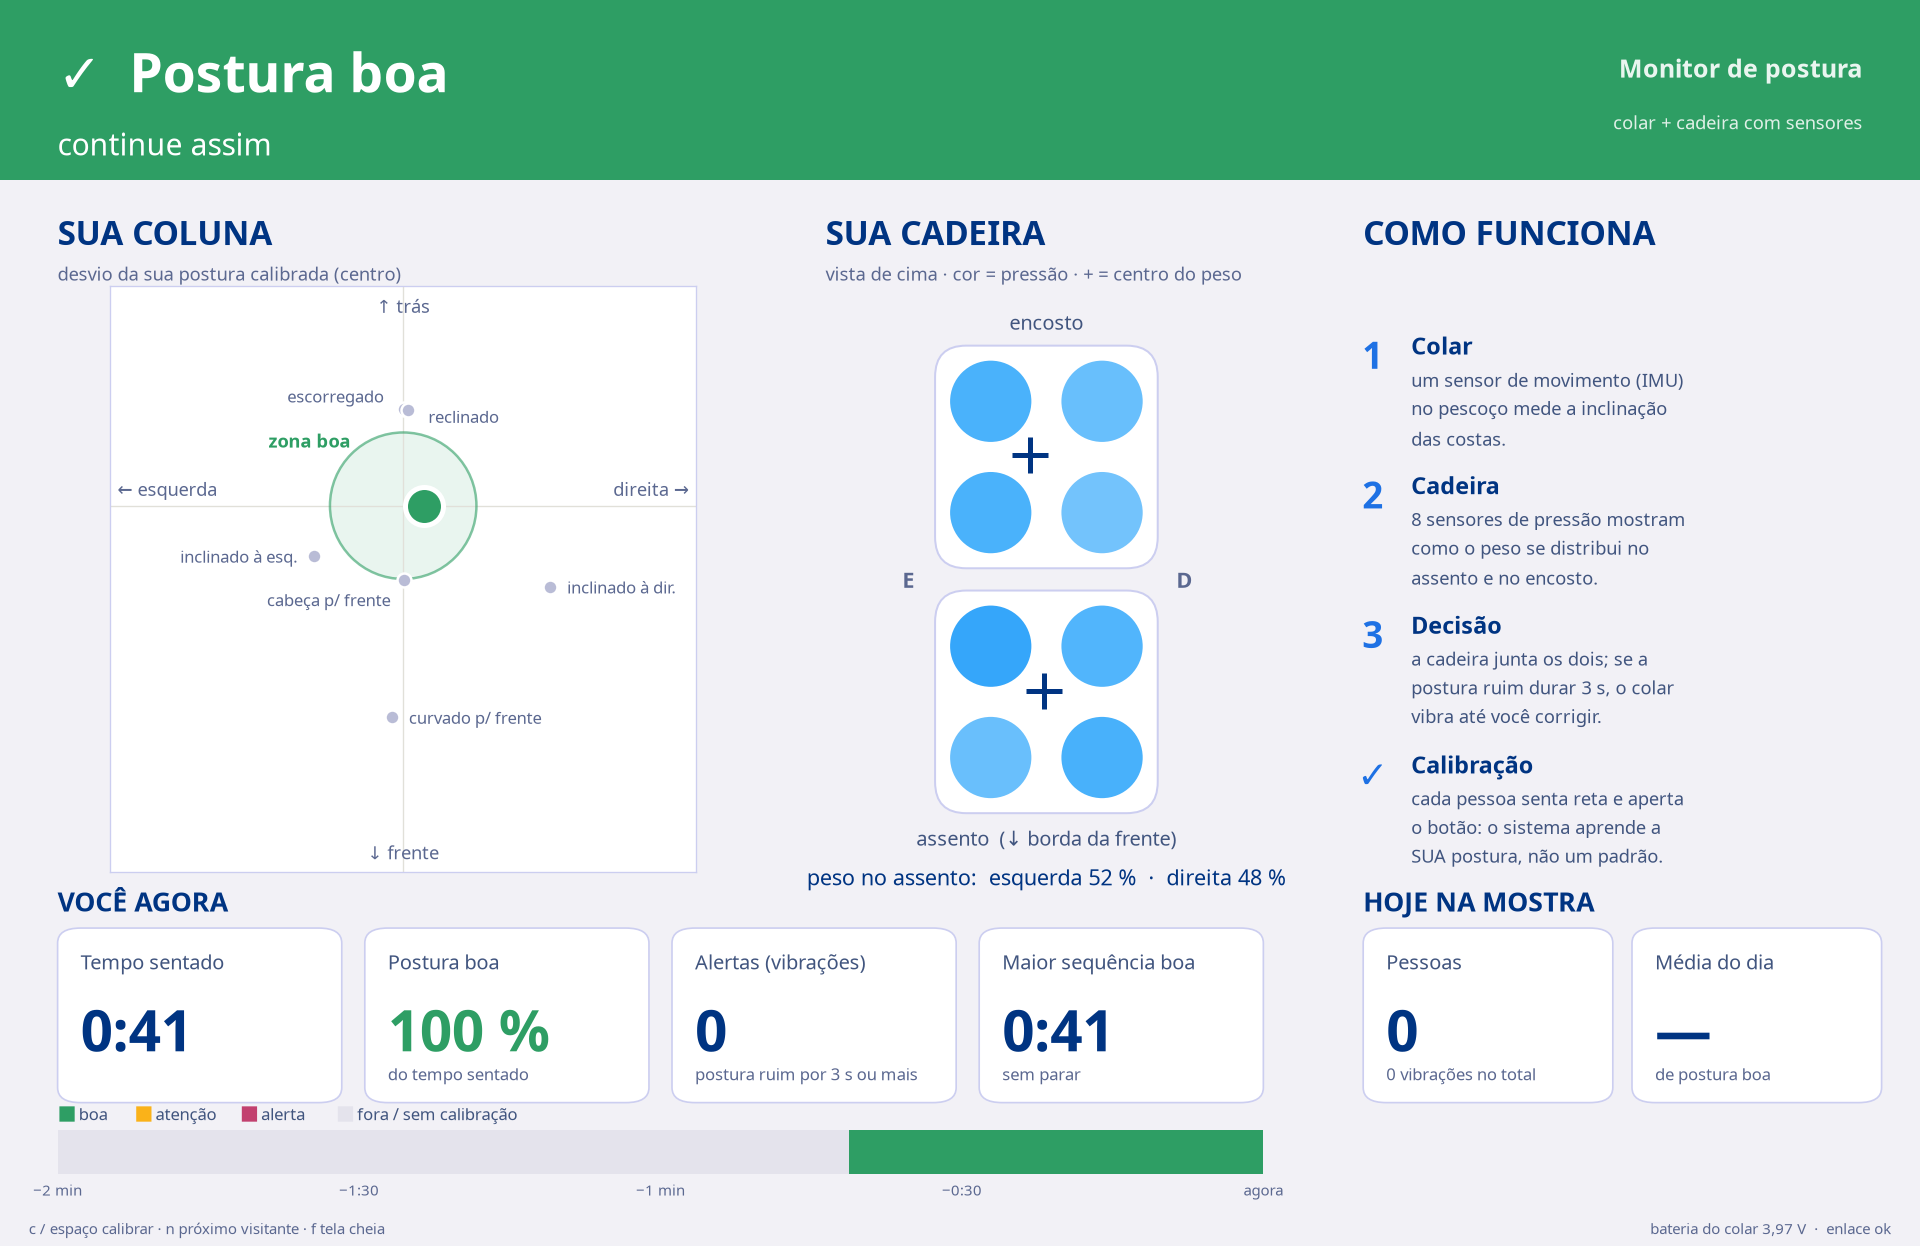
\includegraphics[width=\linewidth]{met-dashboard-boa.png}
  \fonte{Elaborado pelo autor (2026), captura disponível em \texttt{docs/stand}}
\end{figure}

O modo padrão prioriza USB, passa ao BLE após desconexão ou 1\,s
sem dados USB válidos e retorna ao cabo quando os dados reaparecem.
Somente uma fonte alimenta a tela a cada instante; no modo automático,
usa-se o relógio monotônico do notebook para manter a continuidade da
visita. Em BLE, a calibração depende do botão físico. A interface
tolera intervalos de até 2\,s para sua contabilização visual e
aguarda 5\,s de silêncio BLE para mostrar desconexão. Essa
continuidade estimada não recupera amostras perdidas. O modo
\texttt{--replay} reproduz CSVs sem hardware e mantém os contadores
da reprodução separados do dia real.

\subsubsection{Toolchain e testes automatizados}

Os programas embarcados são compilados com \texttt{arduino-cli},
core \texttt{Seeeduino:nrf52} versão 1.1.13 e alvo
\texttt{Seeeduino:nrf52:xiaonRF52840Sense}. A biblioteca local é
incluída por \texttt{--libraries firmware/libraries};
\texttt{Adafruit\_TinyUSB} acompanha o core. Para a bancada FSR
histórica utilizou-se o alvo \texttt{arduino:avr:uno}. As placas são
selecionadas para gravação por número de série USB, evitando depender
da numeração variável das portas.

A verificação automatizada tem três níveis. Primeiro, testes C++
exercitam protocolo, sequência, validade, portões temporais, bateria,
leitor inercial e formatação serial. Segundo, os próprios programas
\texttt{body.ino} e \texttt{chair.ino} são compilados no computador
com substitutos de rádio, USB e IMU; \texttt{test\_system} executa
ambos sobre um enlace simulado. São exercitados perda de enlace,
reinicialização, duplicatas, host USB que deixa de ler e falhas
retornadas pelo barramento. Terceiro, testes Python verificam
carregadores, análise, leitores de transporte e sessões do dashboard.

O teste C++ \texttt{test\_fusion} compara motivo e alerta, amostra a
amostra, com trechos reais cujo resultado esperado foi gerado por
\texttt{analysis/fusion.py}. As bases e o estado inicial do portão
acompanham os trechos em \texttt{fusion\_cases.txt}. Os testes Python
também verificam a equivalência entre replay sequencial e vetorizado
e a leitura de saídas do sistema simulado. Essa comparação confere a
transposição da regra para C++; não constitui validação independente
dos limiares nos usuários.

O \texttt{Makefile} de \texttt{firmware/test} usa C++11, avisos como
erros e sanitizadores de endereço e comportamento indefinido. Há um
teste adicional com \texttt{-Ofast}, opção do core que pode eliminar
verificações usuais de \texttt{NaN}; por isso o protocolo inspeciona a
representação IEEE-754 dos números. Os comandos de reprodução são
\texttt{make -C firmware/test} e, para a suíte Python,
\texttt{QT\_QPA\_PLATFORM=offscreen} seguido de
\texttt{.venv/bin/python -m unittest discover -s analysis}.
Os substitutos em host não reproduzem um barramento físico travado
nem todos os aspectos temporais do microcontrolador, devendo ser
complementados pela observação em hardware.

\subsection{Procedimentos experimentais e avaliação}
\label{sec:met-experimentos}

\subsubsection{Caracterização em bancada: Campanhas A e B}

Na etapa parcial, realizada em junho de 2026, os canais foram
caracterizados separadamente. A Campanha A empregou um participante
com o XIAO sem o colar/invólucro final, fixado abaixo do pescoço e
conectado por USB. Registraram-se posturas mantidas por aproximadamente
10\,s, com movimentos rotulados e excluídos da análise. Retiradas e
recolocações do sensor, seguidas de calibração, permitiram avaliar a
dependência da referência em relação à montagem. Os scripts de
validação e visualização estão em \texttt{analysis/archive}.

A codificação dessa campanha foi distinta da integrada: 0 indicava
ereto; 1, curvar para a frente; 2 e 3, inclinações laterais; 4,
cabeça baixa; 5, recostar com quadril à frente; e 9, transição.
Não se equiparou automaticamente essa última postura à reclinação
apoiada definida no protocolo final. A série registrada utilizou
posturas pronunciadas, não representando uso natural contínuo.

A Campanha B utilizou Arduino Uno, FSR402 e divisor com resistor
medido de 2833\,\ohm, alimentado a 5\,V, com ADC de dez bits.
Foram caracterizadas três peças físicas, com carga aplicada por
elemento rígido centralizado sobre o sensor e lida em balança.
O protocolo de precisão incluiu níveis próximos de 50, 100, 200, 400,
800, 1200, 1600 e 2000\,g, em subida e descida, retenção de cerca
de 5\,s por nível e ensaio de deriva sob massa constante próxima
de 1\,kg, planejado por 10\,min.

O tratamento recuperou resistência a partir do divisor, reuniu níveis
com pequenas oscilações da carga digitada e comparou medianas,
trajetórias de carga/descarga, condutância e modelos de resposta.
As capturas passaram pelo validador \texttt{validate\_fsr.py}.
Esses ensaios caracterizam sensores e montagem de bancada, não
calibram força na espuma da cadeira integrada. Os resultados de
ambas as campanhas são apresentados na Seção~\ref{sec:resultados}.

\subsubsection{Capturas integradas de 21 de outubro de 2026}

O conjunto de desenvolvimento contém nove arquivos de oito sujeitos,
com duas sessões de um mesmo participante mantidas sob a mesma
identidade. Os CSVs reúnem IMU e FSRs em um único relógio de recepção
da cadeira. O motor foi mantido mudo nas capturas de desenvolvimento,
para não orientar a autocorreção do participante nem introduzir
vibração na aquisição. Na ocasião, usou-se uma compilação com motor
silenciado; o mecanismo em execução \texttt{--motor-muted}, descrito
anteriormente, foi acrescentado depois e é o procedimento atual.
Não se atribuem retroativamente colunas da versão 5 aos logs de
21/10, identificados com protocolo 4.

A Tabela~\ref{tab:met-posturas} apresenta a codificação integrada.
O operador marca 0 antes de qualquer movimento e só seleciona a
postura após sua estabilização. As tags persistem até a próxima
tecla; descrevem a instrução dada ao participante e não uma medida
anatômica independente.

\begin{table}[H]
  \centering
  \begin{singlespace}
  \caption{Tags e posturas do protocolo do sistema completo.}
  \label{tab:met-posturas}
  \small
  \begin{tabularx}{\linewidth}{@{}c l X@{}}
    \toprule
    Tag & Postura & Instrução operacional \\
    \midrule
    0 & Transição & Movimento ou trecho não rotulado; excluído da pontuação. \\
    1 & Ereto & Sentar até o fundo, na postura de referência da calibração. \\
    2 & Curvado à frente & Curvar o tronco, retirando as costas do encosto. \\
    3 & Cabeça à frente & Manter o tronco apoiado e projetar cabeça/pescoço à frente. \\
    4 & Escorregado & Deslocar o quadril à frente, mantendo apenas as escápulas no encosto. \\
    5 & Inclinado à esquerda & Inclinar o tronco para a esquerda, apoiado no braço. \\
    6 & Inclinado à direita & Repetir a inclinação para a direita. \\
    7 & Reclinado & Apoiar o encosto inteiro, conservando o quadril atrás; aceitável. \\
    8 & Perna E sobre D & Cruzar a esquerda sobre a direita, com tronco ereto. \\
    9 & Perna D sobre E & Cruzar a direita sobre a esquerda, com tronco ereto. \\
    \bottomrule
  \end{tabularx}
  \end{singlespace}
  \fonte{Elaborado pelo autor (2026), a partir de \texttt{docs/protocolo-captura.md}}
\end{table}

O protocolo curto prevê aproximadamente 15\,s por postura e
10\,s de ereto entre posturas, duas passadas em ordem embaralhada,
série sutil e recolocação com nova calibração. Voltar o quadril ao
fundo depois de escorregar é uma instrução explícita para evitar
posturas combinadas. A ordem embaralhada busca separar efeitos de
postura dos efeitos de tempo, acomodação e deriva.

Entretanto, o registro de execução não sustenta que todos completaram
esse roteiro. As primeiras sessões foram séries marcadas em ordem
fixa; algumas tiveram uma passada, outras duas e recalibrações.
Somente as sessões de Gustavo e Rafael utilizaram a primeira passada
das folhas embaralhadas P1 e P2, respectivamente, com omissões
registradas na segunda. Por isso, a avaliação usa os segmentos
efetivamente disponíveis, sem supor um desenho balanceado, séries
sutis completas ou recolocações sistemáticas para os oito sujeitos.

Antes da análise, tomou-se o mapa corrigido para a perspectiva de
quem senta: os cabeçalhos de 21/10 haviam sido mapeados de frente
para a cadeira e tiveram esquerda/direita espelhadas, com nota de
proveniência. O registro também documenta correções pontuais de tags
e a separação de uma sessão anexada por engano a outro arquivo.
Preservaram-se as observações de deriva e de posturas mistas para
interpretar os limites do conjunto. Não se aplicou estatística
inferencial aos oito sujeitos.

\subsubsection{Reconstrução das calibrações e replay da decisão}

O carregador \texttt{captures.py} lê dados, eventos iniciados por
\texttt{\#}, mapa dos FSRs, tags e identificadores de calibração.
Quando a linha de base dos FSRs está gravada no evento de calibração,
ela é utilizada diretamente. Nos logs anteriores, reconstrói-se a
janela de 20 amostras: as 19 linhas anteriores a
\texttt{\# calibrated} e a primeira posterior, já com o novo
\texttt{calid}. Isso reproduz o instante em que a cadeira termina
a média e só então escreve a linha correspondente.

Verificam-se comprimento da janela, presença do evento inicial,
continuidade da sequência, sessão corporal e validade da IMU. Se
faltam linhas ou a janela é incoerente, a calibração é marcada como
não confiável e não participa da pontuação. Para uma calibração já
ativa antes do início do arquivo, sem evento disponível, usam-se as
primeiras 20 linhas daquele identificador como aproximação da base.
Esse recurso afeta os trechos iniciais não rotulados; uma base que
seria recusada pela regra final não habilita a avaliação.

O replay percorre cada sessão completa na ordem temporal original,
usando milissegundos inteiros da cadeira. Reaplica referências,
reinícios, pausas de captura e o portão temporal amostra a amostra.
Os trechos de transição continuam alimentando o estado da regra:
excluí-los do processamento alteraria a contagem dos 3\,s e a
histerese. Durante uma captura de referência, conserva-se o estado
do portão sem atualizá-lo, como no programa embarcado.

Um cuidado adicional distingue rejeição real e contrafactual. A
cadeira preserva a referência anterior se recusar uma nova captura.
Ao simular a recusa de uma calibração que o firmware antigo aceitou,
o replay não utiliza os desvios já registrados sob aquela referência
como se pertencessem à anterior; deixa esses trechos sem decisão
avaliável. Comparam-se as regras somente nas linhas calibradas com
base confiável e utilizável pela fusão final.

Para a pontuação, consideram-se as tags diferentes de 0 e descartam-se
os primeiros 2\,s após cada troca de tag. A expressão ``amostras
assentadas'' designa aqui esse recorte temporal estabilizado, não
uma seleção de acertos pelo estado previsto pelo detector. Cada
segmento é uma sequência contínua de uma tag, sob os critérios de
calibração válidos. O replay vetorizado acelera a busca, com
equivalência ao sequencial verificada pelos testes.

\subsubsection{Métrica, grade de candidatos e validação por sujeito}

As tags 2--6 integram o grupo com alerta esperado; 1, 7, 8 e 9
integram o grupo sem alerta esperado. Para cada segmento $s$, calcula-se
$a_s$, a fração das suas amostras estabilizadas avaliáveis em que o
alerta está ativo. A função de escolha é
\begin{equation}
 J=\frac{1}{2}\left[
 \frac{1}{|\mathcal{B}|}\sum_{s\in\mathcal{B}}a_s+
 \frac{1}{|\mathcal{A}|}\sum_{s\in\mathcal{A}}(1-a_s)
 \right],
 \label{eq:met-pontuacao}
\end{equation}
em que $\mathcal{B}$ reúne os segmentos ruins e $\mathcal{A}$, os
aceitáveis, incluindo pernas cruzadas. Trata-se da média entre
sensibilidade temporal média dos segmentos ruins e especificidade
temporal média dos aceitáveis. Cada segmento tem o mesmo peso dentro
do grupo; a função não é a fração global de amostras corretas nem a
proporção de segmentos em que ocorreu ao menos um disparo.

A busca em \texttt{fusion.py} compreende 2250 combinações:
\begin{itemize}[nosep]
  \item \texttt{ALERT\_DEG} em $\{8,9,10,11,12\}\degree{}$;
  \item \texttt{SLUMP\_FRAC} desabilitado ou em $\{0{,}2;\,0{,}3;\,0{,}4;\,0{,}5\}$;
  \item \texttt{RECLINE\_FRAC} em $\{0{,}5;\,0{,}6;\,0{,}7;\,0{,}8;\,0{,}9\}$
        ou desabilitado;
  \item \texttt{LEAN\_DEG} em $\{5,6,7,8\}\degree{}$ ou desabilitado;
  \item \texttt{LEAN\_LR} em $\{0{,}03;\,0{,}05;\,0{,}08\}$.
\end{itemize}
Mantêm-se \texttt{CLEAR\_DEG} igual a \texttt{ALERT\_DEG} menos $3\degree{}$
e permanência de 3\,s. A seleção utiliza a média da pontuação de
cada candidato e dos vizinhos a até um passo em cada eixo da grade,
para privilegiar regiões estáveis do espaço de parâmetros.

Aplicou-se validação deixando um sujeito de fora
(\emph{leave-one-subject-out}, LOSO): selecionam-se parâmetros com
sete sujeitos e avalia-se o oitavo, repetindo-se a separação por
identidade. As duas sessões de André permanecem juntas na mesma
dobra. Compara-se também a regra histórica somente inercial,
representada por \texttt{CURRENT}, com os termos FSR desligados.
Esse nome no script é histórico; a regra embarcada final é a fusão.
Uma seleção feita com todos os oito sujeitos é identificada como
ajuste no próprio conjunto, separadamente da avaliação LOSO.

Além da pontuação, os scripts produzem fração de tempo alertado por
postura, ocorrência de alerta por segmento e latência a partir da
marcação da tag. Essa latência não mede diretamente o atraso desde o
início físico do desvio: o participante pode ter assumido a postura
durante a transição, antes da tecla. A comparação entre replay e
coluna de alerta gravada também considera o arredondamento dos
ângulos a uma casa decimal. Resultados e divergências são reservados
à Seção~\ref{sec:resultados}.

\subsubsection{Validação em hardware em 22 de outubro de 2026}

A regra de fusão foi gravada nas duas placas e exercitada com motor
ativo. Foram registradas duas sessões, sendo uma de André, já
presente no desenvolvimento, e uma de Lucas, primeiro sujeito novo.
A sessão de André utilizou a revisão \texttt{c4ae8f2}, em sequência
guiada, com retornos ao ereto, assento vazio, recolocação e nova
calibração. A de Lucas utilizou \texttt{b3c29b1}, protocolo 5,
com execução parcial da folha P3: tags 1, 5, 4, 8, 1, 2 e 6,
seguidas de aproximadamente 10\,s de cadeira vazia. Não foram
executadas nessa sessão as tags 3, 7 e 9, a segunda passada, a série
sutil ou a recolocação.

O procedimento verificou aquisição integrada, decisão transmitida,
vibração e retorno após correção, conservando o CSV para inspeção.
Somente o participante novo permite uma observação adicional fora
do conjunto usado na seleção, ainda limitada às posturas realizadas.
A identificação da cadeira e os detalhes de montagem do
colar/invólucro não foram registrados nessas sessões.

Esses arquivos foram obtidos antes da alteração que retém a última
orientação sem vibração, descrita na Seção~\ref{sec:met-corpo}.
O histórico \texttt{5e82e20}, seguido de \texttt{6eaafbe}, documenta
a introdução dessa proteção e o limite final de 1{,}5\,s.
Assim, o ensaio de 22/10 avalia a implementação que estava gravada
na ocasião; não é tratado como novo ensaio de hardware da correção
posterior. Uma repetição computacional dos ângulos retidos deve ser
identificada como simulação, sem substituir uma nova captura.

\subsubsection{Demonstração na feira de ciências}

Em novembro de 2026, o sistema completo foi demonstrado informalmente
a dezenas de pessoas, com calibração individual, observação da tela
do \texttt{mostra.py} e retorno vibratório. O fluxo consistiu em
colocar o colar, sentar até o fundo, calibrar pelo botão e demonstrar
curvatura, inclinação lateral, escorregamento, reclinação apoiada e
pernas cruzadas. O encerramento da visita e a limpeza da referência
preparavam o sistema para a próxima pessoa.

Essa atividade avaliou a operação pública do conjunto, com sensores,
atuador, alimentação e interface. Não houve sessões rotuladas ou
registro de dados experimentais para estimar sensibilidade,
especificidade ou taxa de acerto. Os contadores de demonstração do
dashboard não foram adotados como base quantitativa do relatório.
A feira é, portanto, distinguida das capturas controladas e da
avaliação por replay.

% REFERENCIAS NOVAS:
% Nenhuma referência bibliográfica externa nova. Os parâmetros e os
% procedimentos foram extraídos dos fontes, protocolos e registros
% versionados do próprio projeto, identificados no texto.
